\cotefile{21}
\scanpage{17}

% vertical rule at the left of the four lines
Si $X$ est loc noeth \unsure{quelct|quelcque|quelcq|quelconque} seulement, on dit que $F$ a la propriété $(P_1)$ (\unsure{resp\textsuperscript{t}|resp.} $(P_2)$). en un pt $x\in X$, si $\mathrm{Loc}_x(F)$ sur $\mathrm{Loc}_x(X)$ a la propriété $(P_1)$ resp. $(P_2)$.

\uline{Proposition} 3\quad Soit $X$ un espace loc. noeth. spectral, $Y$ une partie fermée de $X$, $F$ un faisceau d'ens sur $X$. Conditions équivalentes

(i) $F$ a la propriété $P_1$ (resp. $P_2$) rel à $Y$

(ii) Pour tt $x\in Y$, $F$ a la propriété $P_1$ (resp. $P_2$) en $x$.

\uline{Démonstration}\quad On peut supposer $X$ affine.

\deleted{\unsure{a)|$\alpha$)} \uline{\unsure{Cas de}} $(P_1)$} Prouvons d'abord le

\uline{Corollaire} 4\quad Si $F$ satisfait à la condition $P_1$ $(P_2)$ rel. à $Y$, alors pour tt ouvert $X'\subset X$ et toute partie fermée $Y'$ de $X'$ telle que $Y'\subset X'\cap Y$, $F':=F\mid X'$ satisfait $P_1$ $(P_2)$ rel à $Y'$.

% slanted
\margin{n'utilise pas l'hyp loc. noeth. sur $X$}

\inserted{Soit $U'=X-Y$.} On peut supposer évidemment $X'=X$. Soit $U$ un ouvert quelconque de $X$,

% archive sheet number: 16
\scanpage{18}

\deleted{Pour} Cela résulte du

\uline{Lemme}\quad Pour que deux parties loc. constructibles $E,E'$ de $X$ \deleted{\unsure{coïncident}} \inserted{\unsure{satisfassent} $E\supset E'$} au voisinage de $x$, il f. et s. que \deleted{leurs \unsure{traces} $\unsure{E_{(x)}|E_{(x)}'}\supset E\unsure{'|.}$} l'on ait $E_{(x)}\supset E'_{(x)}$.

Introduisant \deleted{$\unsure{E|E''}$} $Z=E'\cap\complement E$, on est amené à montrer que si $Z$ constructible est tel que $Z_{(x)}=\emptyset$, alors $\overline Z\not\ni x$ i.e. $X-Z$ est un voisinage de $x$. Immédiat....

Cela prouve que $\unsure{\alpha|a}$ est injectif. Prouvons qu'il est \uline{surjectif}. \inserted{Soit $f\in\Gamma(V_{(x)},F_{(x)})$} Pour tt $y\in V_{(x)}$, soit $W^y$ un voisinage ouvert de $y$ \inserted{ds $X$}, et $f^y\in\Gamma(W^y,F)$, tels que $(f^y)_{y'}=f_{y'}$ \deleted{pour} $y'\in W^y\cap \unsure{V_{(x)}|X_{(x)}}=(W^y)_{(x)}$

\figure{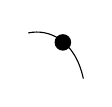
\begin{tikzpicture}[x=1cm,y=1cm]
\draw (0,0.43) .. controls (0.28,0.49) and (0.60,0.32) .. (0.70,-0.15);
\fill (0.44,0.31) circle (0.105);
\end{tikzpicture}}

\margin{$V_{(x)}\subset X_{(x)}$}

\deleted{Les $W^y$ recouvrent $V_{(x)}$, donc un nb fini \unsure{recouvrent}, i.e. \illegible{2} des ouverts $W_i$ \unsure{avec}}

\deleted{Pour $y'\in V_y$ voisin de $y$ on aura alors $(f^y)_{y'}=f_{y'}$, donc \unsure{à} à condition de restreindre le voisinage \unsure{de} $W^y$, on peut supposer que \unsure{ceci} \unsure{est fait}.}

Les $W^y$ recouvrent $V_{(x)}$ qui est qu. cpt, il existe un nb fini des $W^y$ qui recouvrent, donc \deleted{\unsure{des}} un nb fini

% archive sheet number: 17
\scanpage{19}

On a alors le diagramme commutatif

\diagram{\begin{tikzcd}[ampersand replacement=\&]
\Gamma(V,F) \arrow[r,"\rho'"] \arrow[dr,swap,"\rho"] \& \Gamma(V\cap U',F) \arrow[d,"\rho''"] \\
\& \Gamma(V\cap U,F)=1
\end{tikzcd}}

Si $F$ satisfait à $P_1$ ($\deleted{\unsure{\mathrm{rel}}}P_2$) rel. à $Y$, alors $\rho$ et $\rho''$ sont \deleted{\unsure{des}} inj (bijectifs) puisque $V\cap U=(V\cap U')\cap U$, donc \deleted{leur composé $\rho$ l'est, ce qui} $\rho'$ est inj. (bijectif) ce qui prouve le corollaire.

\deleted{\uline{\unsure{Dém. de prop.} 3 pour $P_1$}}

\uline{Lemme} 5\quad On a, pour tt $x\in X$, \deleted{\unsure{désignant}} \inserted{et tt ouvert $V$,} \deleted{\unsure{posant} $\unsure{U}\ \mathrm{Loc}'_x(X)=\mathrm{Loc}_x(X)-\{x\}$,} $X_{(x)}=\mathrm{loc}_{\deleted{\unsure{x}}x}(X)$, \deleted{$X'_x=X_x-\{x\}$} $\deleted{\unsure{U}}V_{(x)}=\deleted{\unsure{U}}V\cap X_{(x)}$, l'isom. \unsure{suivant}

\[
\deleted{\Gamma(X_x,F)\simeq F_x,\quad \Gamma(\unsure{X'_x|\check X'_x}}
\]

\[
\Gamma(V_{(x)},F_{(x)})\xleftarrow{\sim}
\underset{\substack{W\ \text{voisinage}\\\text{ouvert de }x}}{\varinjlim}\ \Gamma(W\cap V,F)
\tag*{$(*)$}
\]

On a un hom évident, prouvons qu'il est bijectif. Soit $f,g\in\Gamma(W\cap V,F)$ qui \unsure{devient|deviennent} \deleted{\unsure{nulle|nuls}} \inserted{égaux} sur $V_{(x)}$, donc ils sont \unsure{nulle|nuls|nulles} dans un voisinage ouvert \inserted{$E$} de $V_{(x)}\subset X$, \deleted{soit $\unsure{V'_x|W'_x}\ \unsure{E,|E'}$} je dis que $E$ contient un ens. de la forme $W'\cap V$, $W'$ vois. ouvert de $x$.

% archive sheet number: 18
\scanpage{20}

Prouvons $(\mathrm{ii})\Longrightarrow(\mathrm{i})$. La question étant locale sur $X$, on peut supposer $X$ \uline{noethérien}.

On prouve par récurrence noethérienne que pour tte partie fermée $Y'$ de $Y$, $F$ a la propriété $P_1$ $(P_2)$ rel. à $Y'$, on peut supposer que pour tt $Y'$ fermé $\subset Y$, $Y'\ne Y$, $F$ a déjà la propriété en question \inserted{rel. à $Y'$} et se borner à prouver que $F$ a la propriété $P_1$ $(P_2)$ rel. à $Y$ dans ce cas.

\deleted{\unsure{Si|Le} $Y=\emptyset$, c'est trivial, sinon soit $\deleted{y}\inserted{x}$ un pt \uline{maximal} de $Y$.} On est ramené à \deleted{prouver que}, prouver que

\[
\Gamma(X,F)\longrightarrow\Gamma(\deleted{\unsure{X}}U,F)\qquad (U=X-Y)
\]

est injectif (bijectif). Soient $f,g\in\Gamma(X,F)$ ayant $=$ image dans $\Gamma(U,F)$, prouvons qu'ils sont identiques\unsure{;|,} \deleted{il suffit d'établir que \unsure{de se dire que} pour tt $x\in Y$, $f_x=g_x$ ; si $\overline x\ne Y$,}

% slanted
\margin{\deleted{\unsure{injectivité} \unsure{du|de} \illegible{1} \unsure{5}}}

\unsure{Cela.|Ceci.|local.} Tout d'abord, en vertu \deleted{\unsure{du lemme 5}} \inserted{et de l'hyp. $P_1$ \uline{en $x$}} ils sont identiques en $x$, donc au voisinage de $x$, et on achève par l'hyp. de récurrence.

Soit \unsure{Mainten\deleted{ant}|Maintenant} (\unsure{ds|sous|et} l'hyp $P_2$ en les $x\in Y$)

% archive sheet number: 19
\scanpage{21}

d'ouverts $W_i$ \deleted{de} $X$ recouvrant $V_{(x)}$ \inserted{(donc en vertu du lemme on peut supposer qu'ils recouvrent $V$)} et des $f_i\in\Gamma(W_i,F)$, \unsure{telles|tels} que $y\in W_{ix}\deleted{\unsure{V_{(x)}|V_x}}\Rightarrow f_{iy}=f_y$.

Soit \deleted{$\unsure{f}$} $W'_{ij}$ l'ens des $y\in W_i\cap W_j=W_{ij}$ tels que $f_{iy}=f_{jy}$. Cet ens \deleted{est} \inserted{est ouvert et} contient $W_{ij}\cap V_{(x)}=W_{ij\,x}$

Par le lemme \deleted{\unsure{préc.}} déjà cité, \unsure{rapetissant} $X$ \deleted{$W\cap V$} autour de \deleted{$\unsure{(x)}$}$x$, on peut supposer que $W'_{ij}=W_{ij}$. Alors on dispose d'une vraie section. OK ....

% slanted
\margin{Généraliser \deleted{\unsure{ces}} les lemmes à des procédés de localisation plus généraux.....}

Prouvons maintenant $(\mathrm{i})\Rightarrow(\mathrm{ii})$ : En effet, \unsure{soit|soit le} $x\in Y$, \deleted{\unsure{considérons}} notons que par le \deleted{\unsure{coroll}} corollaire 4, $F$ satisfait à $P_1$ $(P_2)$ rel. à $\overline x$, donc \inserted{posant $V=X-\overline x$,} on a pour tt voisinage ouvert $W$ de $x$

\[
\Gamma(W,F)\longrightarrow\Gamma(W\cap V,F)
\]

est inj. (bij), donc

\[
\underset{W}{\unsure{\underline{\lim}|\varinjlim}}\ \Gamma(W,F)\mathrel{\unsure{-|\to}}\Gamma(W\cap V,F)
\]

est injectif (bij) or cet hom s'identifie à

\[
\Gamma(X_{(x)},F_{(x)})\longrightarrow\Gamma(X'_{(x)},F_{(x)})
\]

en appliquant deux fois le lemme 5, OK.

% archive sheet number: 20
\scanpage{22}

$f\in\Gamma(U,F)$, montrons qu'on peut prolonger $f$ en une section de $f$ sur $X$. Il suffit de prolonger dans un voisinage de $x$, grâce à l'hyp. de récurrence. Or c'est encore possible grâce à l'hyp $P_2$ en $x$, et le lem. 5. (\unsure{injectivité} du \unsure{ledit}). OK.

\uline{Définition} 6\quad Soit $\mathcal F$ une catégorie fibrée sur la catégorie des ouverts d'un espace top. $X$, soit $Y$ une partie fermée de $X$. On dit que $\mathcal F$ satisfait la condition $P_1$ \deleted{$(P_2$} (resp. $P_2$, resp $P_3$) rel. à $Y$, si pour tt ouvert $V\subset X$, le foncteur

% margin note written sideways
\margin{Si $X$ est loc. noethérien \unsure{spectral|spécial}, on dit que $\mathcal F$ satisfait la condition $P_1$ ($P_2$, $P_3$) si elle satisfait la condition $P_1$ ($P_2$, $P_3$) rel à $\{x\}$, où $x$ est le pt fermé.}

\[
\deleted{\Gamma}\mathcal F(V)\mathrel{\unsure{\to|-}}\mathcal F(V\cap U)\qquad(\text{où } U=X-Y)
\]

est fidèle (resp. pleinement fidèle, \unsure{respt|resp.} une équivalence de catégories). On dit que $\mathcal F$ satisfait la condition $P_1$ (resp. $P_2$, resp $P_3$) en un pt $x\in X$, si le foncteur

\[
\underset{W}{\underset{\longrightarrow}{\mathrm{Pseudolim}}}\ \deleted{\unsure{\mathcal F|\{}}\mathcal F(W)\mathrel{\unsure{-|\to}}
\underset{W}{\underset{\longrightarrow}{\mathrm{Pseudolim}}}\ \mathcal F(W-W\cap\overline x),
\]

(où $W$ parcourt les vois. ouverts de $x$, est \deleted{une} fidèle (resp\unsure{t.|.} pl. fidèle, resp\unsure{t.|.} une équivalence).

% archive sheet number: 21
\scanpage{23}

Le premier pt signifie, pour $P_1$ (resp $P_2$) que pour tt ouvert $V\subset X$, et tt couple $\unsure{\xi|\zeta|f},\eta\in\mathrm{Ob}\,\mathcal F(V)$, le faisceau $\underline{\mathrm{Hom}}(\xi,\eta)$ sur $V$ satisfait la condition $P_1$ (resp. $P_2$) rel. à $\deleted{\unsure{\xi}}Y\cap Y$.

La condition $P_3$ signifie que \uline{de plus}, pour tt ouvert $V\subset X$, \deleted{et} tt objet $\xi'\in\mathrm{Ob}\,\mathcal F(V\cap U)$ est isomorphe à un objet de la forme $\deleted{\unsure{\xi'}}\xi\mid V\cap U$ où $\xi\in\mathcal F\unsure{W)|(V)|(W)}$.

Le second pt signifie que le foncteur $\mathcal F(X)\longrightarrow\mathcal F(X-\{x\})$ est fidèle \deleted{(\unsure{une équivalence})} (pl. fidèle, une équivalence) \deleted{\unsure{i.e.}} ou encore \inserted{pour $P_1$ $(P_2)$} que pour tt $\xi,\eta\in\mathrm{Ob}\,\mathcal F(X)$, le faisceau $\underline{\mathrm{Hom}}(\xi,\eta)$ satisfait $P_1$ $(P_2)$, et pour $P_3$, que de \uline{plus} tt objet \deleted{\unsure{de}} $\xi'$ de $\deleted{\unsure{\eta}}\mathcal F(X-\{x\})$ soit isom. à un objet de la forme \deleted{$\unsure{V}$} $\xi\mid X-\{x\}$, où $\xi\in\mathrm{Ob}\,\mathcal F(X)$.

% archive sheet number: 22
\scanpage{24}

Le troisième pt se ramène au premier, si on introduit pour tt $x\in X$ la ``catégorie fibrée localisée'' $\mathcal F_{(x)}$ par la condition que pour tt ouvert \deleted{$\unsure{W}\ \unsure{w}$} \deleted{\unsure{de}} $w$ de $X_x$, on pose

\[
\mathcal F_{(x)}(\unsure{w|W})=\underset{\longrightarrow}{\mathrm{Pseudolim}}\ \mathcal F(W)
\]

où $W$ parcourt les ouverts de $X$ tels que $W_{(x)}\supset\deleted{\unsure{X_x|W}}w$ (ou si on veut, tels que $W_{(x)}=w$). \deleted{En \unsure{particulier}}

On \unsure{notera|note} que avec cette définition, pour tt ouvert $V$ de $X$ et \deleted{$\unsure{\xi,\eta\in\mathrm{Ob}}$} $\unsure{\xi|\zeta|f},\eta\in\mathrm{Ob}\,\mathcal F(\unsure{U|V})$, on aura \inserted{\deleted{\unsure{évidemment|fonctoriellement}}} un isom can

\[
\underline{\mathrm{Hom}}(\xi,\eta)_{(x)}\xrightarrow{\sim}
\underline{\mathrm{Hom}}(\xi_{(x)},\eta_{(x)})
% double rule below and to the right of the closing parenthesis
\]

comme il résulte aussitôt des définitions.

% slanted
\margin{On a une \uline{flèche} \deleted{\unsure{surj.}} \unsure{triviale}, et on constate que c'est un isom \deleted{\unsure{par}} \unsure{sur} les fibres en tt pt $y\in\unsure{X_{(x)}|V_{(x)}}$}

\deleted{\unsure{Dire|N.B.}} La propriété $P_1$ ($P_2,P_3$) de $\mathcal F$ en $x$, \uline{s'énonce aussi en disant que} $\mathcal F_{(x)}$ \uline{sur} $X_{(x)}$ \uline{satisfait à la propriété} $P_1$ ($P_2,P_3$).

En ce qui concerne $P_1$ $(P_2)$ cela signifie aussi que pour tt \deleted{ouv.} \inserted{vois.} $V\deleted{\subset X}$ \inserted{de $x$}, et $\xi,\eta\in\mathrm{Ob}\,\mathcal F(U)$ $\underline{\mathrm{Hom}}(\xi,\eta)$ satisfait à $P_1$ $(P_2)$ en $x$.

% archive sheet number: 23
\scanpage{25}

On voit donc, grâce à la proposition 3, la validité des deux premiers énoncés contenus dans

\uline{Prop} 7\quad Soit $X$ un espace loc. noeth. spectral, $\mathcal F$ une catégorie fibrée sur la catégorie des ouverts de $X$, et \deleted{soit} $Y$ une partie fermée de $X$. \deleted{\unsure{On}} Conditions équivalentes

(i) $\mathcal F$ satisfait à $P_1$ ($P_2,P_3$) rel. à $\unsure{x|Y}$

(ii) Pour tt $x\in Y$, $\mathcal F$ satisfait à $P_{\deleted{\unsure{3}}1}$ ($P_2,P_3$) en $x$.

Reste le cas $P_3$, \deleted{\unsure{donc à prouver}} quand $P_1,P_2$ sont déjà vérifiés. On va prouver le

\margin{$\unsure{\Rightarrow|3}$}

\deleted{$(\mathrm{i})\Rightarrow\unsure{(\mathrm{ii})|\mathrm{ii}|(\mathrm{i})}$}

\uline{Corollaire} \uuline{8}\quad Si $\mathcal F$ satisfait $P_1$ ($P_2,P_3$) rel à $Y$, alors pour \deleted{tt ouvert $X'\subset X$, et} tte partie fermée $Y'\subset \deleted{\unsure{X'|Y}}\unsure{Y|X'}$ \deleted{telle que $Y'\subset Y\cap X'$}, $\mathcal F\deleted{\mid X'}$ satisfait $P_1$ ($P_2,P_3$) rel. à $Y'$.

Déjà fait pour $P_1,P_2$ voyons $P_3$. Voyons le diagramme

% archive sheet number: 24
\scanpage{26}

\diagram{\begin{tikzcd}[ampersand replacement=\&]
\mathcal F(\unsure{U|V}) \arrow[r,"\rho'"] \arrow[dr,swap,"\rho"] \& \mathcal F(V\cap U') \arrow[d,"\rho''"] \\
\& \mathcal F(V\cap U)
\end{tikzcd}}

Par hyp. $\rho''$ et $\rho$ sont des équivalences de catégories, donc $\rho'$ en est une, OK.

\deleted{\unsure{A}}Prouvons $(\mathrm{i})\Rightarrow(\mathrm{ii})$, on applique le cor. 8. à $\overline x$ (pour $x\in Y$). Soit $W$ un voisinage ouvert variable de $\overline x$, on aura

\[
\mathcal F(W)\longrightarrow\mathcal F(W-W\cap\overline x)
\]

une équivalence, donc \deleted{en passant à la} en désignant par $\mathcal H$ l'ens des objets à isom près

\[
\mathcal H(\mathcal F(\unsure{w|W}))\xrightarrow{\sim}\mathcal H(\mathcal F(w-W\cap\overline x))
\]

et en passant à la limite inductive

\[
\mathcal H(\mathcal F_{(x)}(X_{(x)}))\xrightarrow{\sim}
\mathcal H(\mathcal F_x(X'_{(x)}))
\]

O.K.

Prouvons $(\mathrm{ii})\Rightarrow(\mathrm{i})$. On est ramené à prouver que tt $\unsure{\xi|\zeta|f}'\in\mathrm{Ob}\,\mathcal F(U)$ provient

% archive sheet number: 25
\scanpage{27}

d'un $\unsure{\xi|\zeta|f}\in\mathrm{Ob}\,\mathcal F(X)$. À cause de l'unicité déjà acquise, la question est locale sur $X$, on peut supposer $X$ noethérien. Par suite, on peut supposer \deleted{que} (par récurrence noethérienne) que pour tt $Y'$ fermé $\subset Y$ et $\ne Y$, \deleted{\unsure{que l'on}} $\mathcal F$ satisfait $P_3$ rel. à $Y'$.

\deleted{Soit} Si \unsure{on} $Y=\emptyset$, il n'y a rien à prouver. Sinon, soit $x$ un pt maximal de $Y$.

Considérons $\xi'\mid X'_{(x)}$, par hypothèse il provient d'un $\xi_{0_{(x)}}\in\mathrm{Ob}\,\mathcal F_{(x)}(X_{(x)})$ lui-même provenant d'un $\xi_0\in\mathrm{Ob}\,\mathcal F(W)$, où $W$ est un voisinage \deleted{de} ouvert de $x$.

\deleted{On \unsure{a}} Considérons les restrictions de $\xi_0$ et $\xi'$ à $W\cap U=V$, par construction elles \deleted{coïncident} \inserted{deviennent isom} sur $V_{(x)}=\underset{\unsure{\nearrow|\to}}{X}'_{(x)}$, donc (par définition de $\mathcal F_{(x)}$) à condition de prendre $W$ assez petit, on peut supposer qu'ils sont isom. Choisissons un tel isom., on trouve donc un objet

$\xi'_1\in\mathrm{Ob}\,\mathcal F(W\cup U)$ prolongeant $\xi'$. Par l'hyp de récurrence, $\xi'_1$ provient d'un $\xi\in\mathcal F(X)$, on a fini.

% archive sheet number: 26
\scanpage{28}

On voit de $=$

\uline{Corollaire} 10\quad Conditions équivalentes

(i) $\mathcal F$ satisfait à $P_1$ ($P_2,P_3$)

(ii) On a $\underline H^i_Y(F)=0$ pour $i<1$ ($i<2$, $i<3$).

Reste le cas $P_3$, où on a posé

\[
\begin{aligned}
\underline H^2_Y(F)&=\text{faisceau associé du préfaisceau}\\
&\qquad V\rightsquigarrow \unsure{H^1|H1}(V\cap U,F).
\end{aligned}
\]

Or, $(\mathrm{i})\Rightarrow(\mathrm{ii})$ puisque $H^1(V\cap U,F)\simeq H^1(V,F)$ (\unsure{fonctoriellet|fonctoriellemnt} en $V$) et que le faisceau associé à $V\rightsquigarrow H^1(V,F)$ est trivial.

On a $(\mathrm{ii})\Rightarrow(\mathrm{i})$. \deleted{On \unsure{est|sera}} ramené en effet à prouver que tt $\unsure{\xi|\zeta|f}'\in\mathrm{Ob}\,\mathcal F(U)$ provient d'un $\xi\in\mathrm{Ob}\,\mathcal F(X)$. Or, \unsure{à} cause des propriétés d'unicité, c'est \uline{local} sur $Y$, et on procède alors comme dans la dém. de prop. 7, en \deleted{\unsure{tout}} raisonnant en un pt quelconque $x\in Y$.

% archive sheet number: 27
\scanpage{29}

\uline{Cas particulier.} Soit $\deleted{\unsure{\mathcal F|F}}\,\deleted{\unsure{\mathcal F}}F$ un faisceau en groupes (pas néc. \unsure{comm|comm.}) sur $X$. Soit $\mathcal F$ la catégorie fibrée (sur les ouverts de $X$) des fibrés principaux homogènes sous $F$. Soit $Y$ une partie fermée de $X$. Alors

% slanted
\margin{Pas d'hyp. \unsure{noethérienne|noetherienne} sur $X$}

\uline{Proposition} 9\quad \deleted{Pour que} \inserted{Conditions équivalentes}

(i) $\mathcal F$ satisfait $P_1$ ($P_2$) rel. à $Y$

(ii) $F$ satisfait $P_1$ ($P_2$) rel. à $Y$.

(iii) On a $\underline H^0_Y(F)=0$ \deleted{pour $i<1$ ($i<2$) i.e. $i=0$ ($i=0,1$)} \inserted{($\underline H^0_Y(F)=0$ et $\underline H^1_Y(F)=0$)}

En effet, \deleted{on aura} si $\xi_0$ est le fibré trivial sur $X$, alors $F\simeq\underline{\mathrm{Hom}}(\xi_0,\xi_0)$, d'où $(\mathrm{i})\Rightarrow(\mathrm{ii})$. D'autre part, si $\xi,\eta\in\mathrm{Ob}\,\mathcal F(V)$, alors $\underline{\mathrm{Hom}}(\xi,\eta)$ est \uline{loc isom} (comme faisceau d'ens) à $F$, d'où $(\mathrm{ii})\Rightarrow(\mathrm{i})$.

Enfin $(\mathrm{ii})\Leftrightarrow(\mathrm{iii})$ par définition de $\underline H^0_Y(F)$ et $\underline H^1_Y(F)$ comme Ker et Coker de $F\unsure{\longrightarrow|-}i_*i^*F$.

% archive sheet number: 28
